\documentclass[conference]{IEEEtran}
\IEEEoverridecommandlockouts
% The preceding line is only needed to identify funding in the first footnote. If that is unneeded, please comment it out.
\usepackage{cite}
\usepackage{amsmath,amssymb,amsfonts}
\usepackage{algorithmic}
\usepackage{graphicx}
\usepackage{textcomp}
\usepackage{xcolor}
\usepackage{hyperref}
\def\BibTeX{{\rm B\kern-.05em{\sc i\kern-.025em b}\kern-.08em
    T\kern-.1667em\lower.7ex\hbox{E}\kern-.125emX}}
\begin{document}

\title{scSpark: a fast and scalable single-cell RNA sequencing data processing toolkit}

\author{\IEEEauthorblockN{1\textsuperscript{st} Given Name Surname}
\IEEEauthorblockA{\textit{dept. name of organization (of Aff.)} \\
\textit{name of organization (of Aff.)}\\
City, Country \\
email address or ORCID}
\and
\IEEEauthorblockN{2\textsuperscript{nd} Given Name Surname}
\IEEEauthorblockA{\textit{dept. name of organization (of Aff.)} \\
\textit{name of organization (of Aff.)}\\
City, Country \\
email address or ORCID}
\and
\IEEEauthorblockN{3\textsuperscript{rd} Given Name Surname}
\IEEEauthorblockA{\textit{dept. name of organization (of Aff.)} \\
\textit{name of organization (of Aff.)}\\
City, Country \\
email address or ORCID}
\and
\IEEEauthorblockN{4\textsuperscript{th} Given Name Surname}
\IEEEauthorblockA{\textit{dept. name of organization (of Aff.)} \\
\textit{name of organization (of Aff.)}\\
City, Country \\
email address or ORCID}
\and
\IEEEauthorblockN{5\textsuperscript{th} Given Name Surname}
\IEEEauthorblockA{\textit{dept. name of organization (of Aff.)} \\
\textit{name of organization (of Aff.)}\\
City, Country \\
email address or ORCID}
\and
\IEEEauthorblockN{6\textsuperscript{th} Given Name Surname}
\IEEEauthorblockA{\textit{dept. name of organization (of Aff.)} \\
\textit{name of organization (of Aff.)}\\
City, Country \\
email address or ORCID}
}

\maketitle

\begin{abstract}
High-throughput single-cell RNA sequencing (scRNA-seq) data processing pipelines typically adopt multiple modules to transform raw scRNA-seq data to gene expression matrices, including sequence quality control, genome alignment and transcript counting. 
With the drastically increasing of scRNA-seq data size, the processing speed and file input/output (IO) have become a bottleneck of the performance of available tools. 
We took advantage of Apache Spark's in-memory computing and inherent scalability to develop a new Java-based pipeline, named scSpark. 
We combined Spark and our proposed functionalities to implement sequence quality control and transcript counting. 
In order to avoid unneccessary disk access while reading FASTQ files and writing SAM files, we used Java Native Interface (JNI) to deliver FASTQ RDD(Resilient Distributed Datasets)'s data, and then extracted return values to SAM RDD. 
By distributing scRNA-seq data and process tasks in the cluster, the scSpark toolkit can significantly reduce disk access for saving and loading temporary results. 
We build spark's cluster on Aliyun to test scSpark. 
The experimental results indicate that scSpark is more efficient and more scalable than any available tool. 
\end{abstract}

\begin{IEEEkeywords}
scRNA-seq data preprocessing, Apache Spark, cloud computing
\end{IEEEkeywords}

\section{Introduction}
Single cell is the fundamental operative unit of a living organism. In the era of precision medicine, exploring the gene expression at single cell level has become crucial. In the past decade, RNA-seq has been widely used to study gene expression patterns. However, the analysis accuracy of RNA-seq could only reach the average level of the cell population.  Single-cell RNA sequencing(scRNA-seq) essentially reveals the transcriptional status at the single cell level, which provides the basis for subsequent bioinformatics analysis~\cite{Papalexi2018SinglecellRS}. 

High-throughput(HT) scRNA-seq protocols, which enable sequencing thousands of cells simultaneously in a single experiment, have emerged as powerful tools to identify and characterize cell types in complex and heterogeneous tissues~\cite{Zhang2019ComparativeAO}.
% are the most popular strategies currently for scRNA-seq technology~\cite{Zhang2019ComparativeAO}. 
Among them, Drop-seq~\cite{Macosko2015HighlyPG}, inDrop~\cite{Klein2015DropletBF} and 10X\cite{Zheng2017Massively} are the three most widely used protocols. 
Two important barcodes, named cell barcode (CB) and unique molecular identifier (UMI) are introduced in scRNA-seq~\cite{Rosenberg2018SinglecellPO}~\cite{Cao2017ComprehensiveSC}. 
CB, which assigns different sequences to each cell for transcriptional source retrieval after sequencing, greatly increases the total length of sequence and reduces the cost of scRNA-seq~\cite{Macosko2015HighlyPG}~\cite{Klein2015DropletBF}. 
These barcodes allow reads to be demultiplexed after the cells have been assembled for sequencing~\cite{Tian2018scPipe}.
In addition to cell barcodes, UMIs are random oligonucleotide barcodes that are used in scRNA-seq experiments~\cite{Kivioja2012Counting}~\cite{Camara2017Methods}.
By UMI, we could distinguish the same copies located in different molecules from those in the same molecule for PCR amplification ~\cite{Smith2017UMItools}.

In the scRNA-seq experiment, the use of multi-level barcodes presented additional challenges for data processing, which was quite different from traditional bulk RNA-seq and low-throughput scRNA-seq experiments. 
In recent years, researchers have developed multiple scRNA-seq data processing tools, typically implementing steps including sequence quality control, genome alignment, and transcript counting to convert raw scRNA-seq data into a gene expression matrix for further downstream analysis. 
The first step is filtering FASTQ readings with low quality CB based on user-defined thresholds. 
This step eliminates most of the false CBs, greatly improving the accuracy of the CBs that need to be considered for counting and reducing the number of CBs. 
The remaining FASTQ reads will map to genomes using the splice-aware aligner, such as STAR~\cite{Dobin2013STAR} or HISAT2~\cite{Kim2015HISAT}. 
Among them, STAR is the most widely used. A number of popular scRNA-seq data processing tools use STAR for mapping, such as UMI-Tools, CellRanger, zumis, scPipe, and STARsolo. 
Previous baseline studies have shown that STAR is one of the most reliable reference genomic aligner for RNA-Seq analysis~\cite{Baruzzo2017SimulationbasedCB}. 
Next, reads are assigned to genes and count matrices for UMIs are generated.~\cite{Parekh2018zUMIs}. 

Nowadays, there are many tools to preprocess scRNA-seq, among which the most popular is CellRanger~\cite{Zheng2017Massively}, UMI-tools~\cite{Smith2017UMItools} and STARsolo~\cite{Blibaum2019STARsolo}. 
CellRanger is a highly integrated data process software tailored by 10X Genomics for single-cell RNA sequencing analysis and it performs comparatively well on machine with enough CPU and memory resources in the big data set, but did badly in small data set. CellRanger performs best under large data sets among existing tools~\cite{Gao2020Comparison}.
UMI-tools~(\url{https://github.com/CGATOxford/UMI-tools}) is an open source tool with an impressively clear process.
STARsolo~\cite{Blibaum2019STARsolo} has improved the parallelism of sequence mapping and counting procedures, and achieved good performance on a single machine.
It is a pity that all avaliable tools only run on a single machine with slow running speed, and cannot be extended to multiple nodes.

There have been many studies using big data framework like Hadoop~(\url{https://hadoop.apache.org}) and Spark~(\url{https://spark.apache.org/}) to optimize Next Generation Sequencing (NGS) Data Processing. 
Due to more efficiency in utilizing memory computing, Spark is a better big data computing framework than Hadoop's MapReduce~\cite{Dean2008MapReduce, Zaharia2012Resilient}. 
SparkBWA~\cite{Abun2016SparkBWA} and GPF~\cite{Li2018Highperformance} are good frameworks with Spart for improving the efficiency of NGS data processing. 
Falco~\cite{Yang2017Falco} has tried to use Spark in scRNA-seq data preprocessing, but it has two limitations. 

Firstly, Falco can't deal with CBs and UMIs, so it is incompatible with any HT scRNA-seq protocol.
Secondly, Falco only uses Spark to simply concatenate the aligner and the feature quantitative softwares, which does not reduce the amount of disk reads and writes during alignment and transcript counting.
Falco’s operations have lots of redundancy disk access which causes its insufficient utilization of Spark’s in-memory computation well. 

The increase of scRNA-seq datasets require more efficient and faster data processing tools. However, the current scRNA-seq data preprocessing tools were designed without considering of the scalability, which could only run on a single computer and could not be extended to a cluster. From UMI-Tools and CellRanger to STARsolo, parallelism and performance has increased; However, due to the limit of a single machine, all of them have no scalability . 
The traditional single machine serial processing mode has been unable to meet the demand of computing and storage resources for super-large scale scRNA-seq data.
Different with Falco, we enhanced STAR's file I/O interface to reduce redundant disk access.
In the end, to achieve parallel and in-memory computing, scSpark implemented transcript counting by combining Spark function and our algorithm【which?】
Our work utilized Spark system architecture to develop a quick and scalable scRNA-seq data preprocessing tool. 
\section{Method}
\subsection{Overview}
We implemented sequence quality control, genome alignment, and transcript counting based on Spark framework. 
We run program across the cluster and default cache data in memory. 
Single machine's capacity is not sufficient to adapt the increasing scRNA-seq data size and the time to process intermediate files occupies a more significant proportion on total time. 
Therefore, reducing the disk access of intermediate files and improving the upstream data process's scalability is the main way to improve avaliable pipelines. 
ScSpark is based on UMI-tools.
\subsection{Sequence quality control}
\begin{figure}
  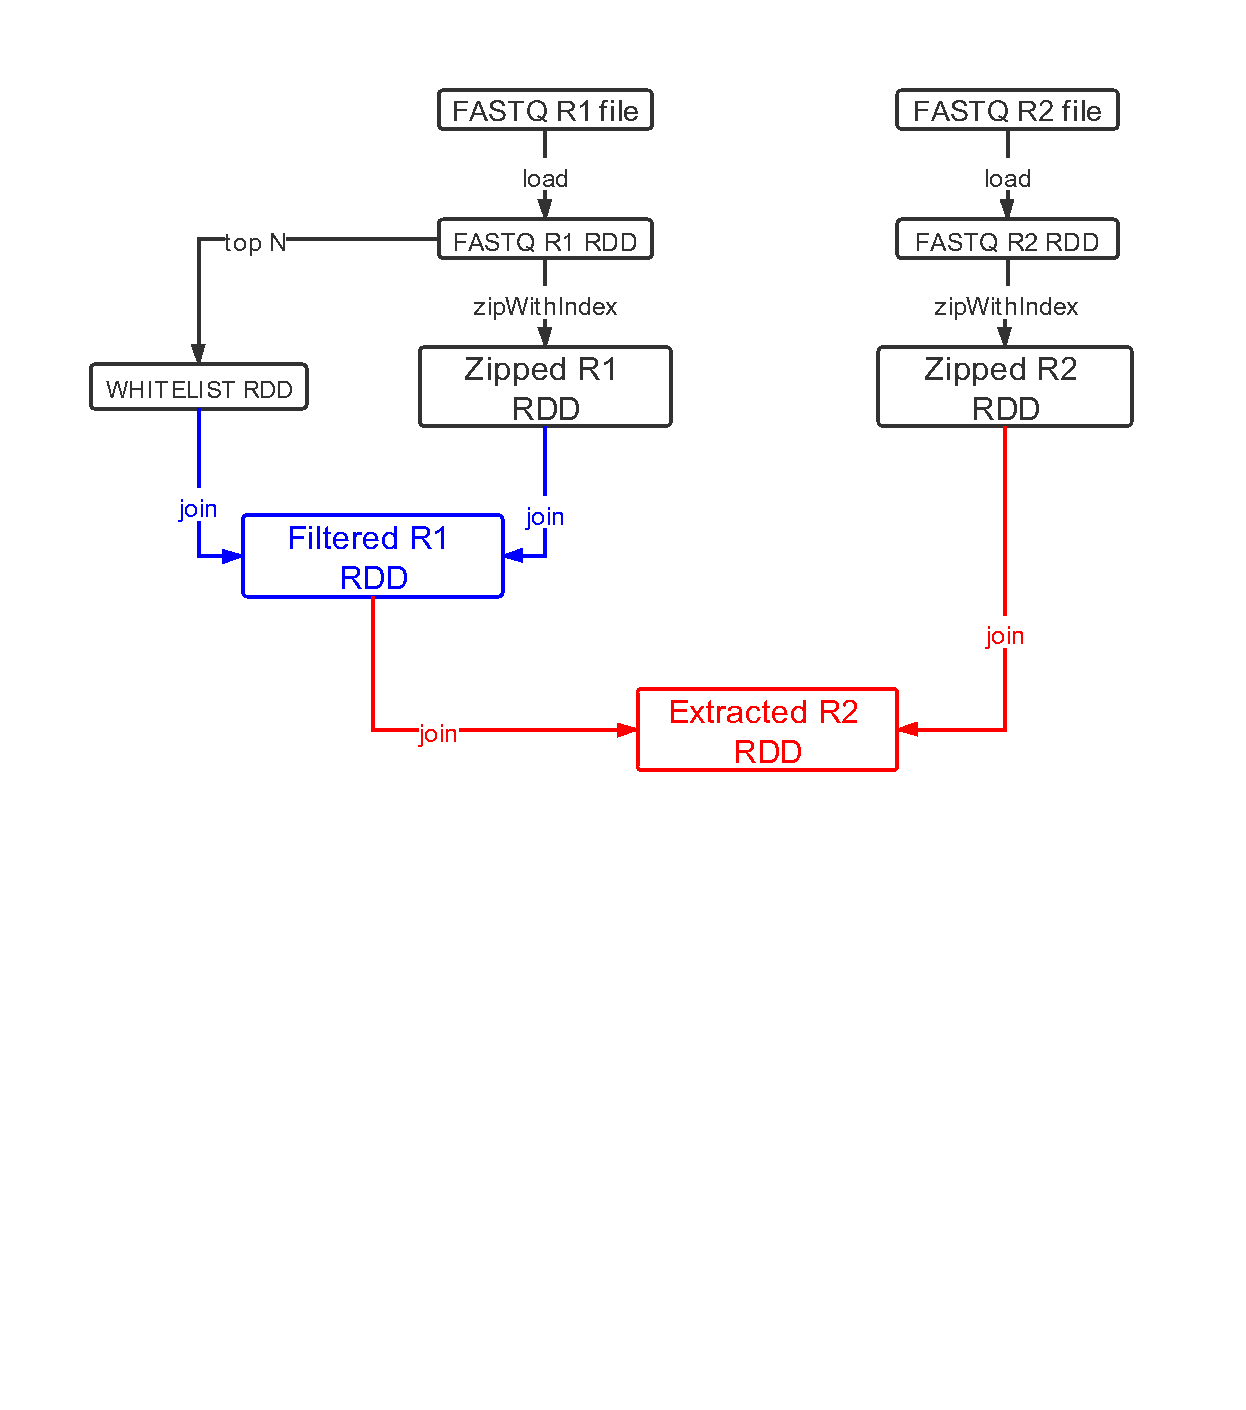
\includegraphics[width=0.5\textwidth]{fig1.pdf}
  \caption{An overview of sequence quality control module based on Spark.} \label{fig1}
\end{figure} 

Large FASTQ files can be loaded in each node's memory parallel and the loading speed doesn't limit by single node disk access speed. 
As shown in Fig~\ref{fig1}, the sequence quality control step typically consists of two main components, i)generating a whitelist including identities of the true cell barcodes is unknown and ii)filtering FASTQ R1 with the whitelist and extracting FASTQ R2 according to filtered FASTQ R1's index.

We loaded each file splits of FASTQ R1 to memory, and abstract them as FASTQ R1 RDD. 
Then we calculated the number of occurences for each CB and selected the most frequent CBs, named whitelist RDD, as intermediate results. 
By using reduceByKey function, each barcode could be counted parallelly in each split of FASTQ R1 RDD and we coould merge each split's result in the end. 
After that we can use the result to generate whitelist RDD by Spark's sort and take function, both of which can parallelly compute in the cluster. 
The filtered FASTQ R1 RDD could be easily got by using the join function to find which read's cell barcode is in the whitelist RDD. 
And then we used filter function to extract FASTQ R2 RDD. 
The last step in sequence quality control was using join function again to combine filtered FASTQ R1 RDD and FASTQ R2 RDD with the same index. 

\subsection{Eleminate redundancy disk access in aligmnent}
\begin{figure}
  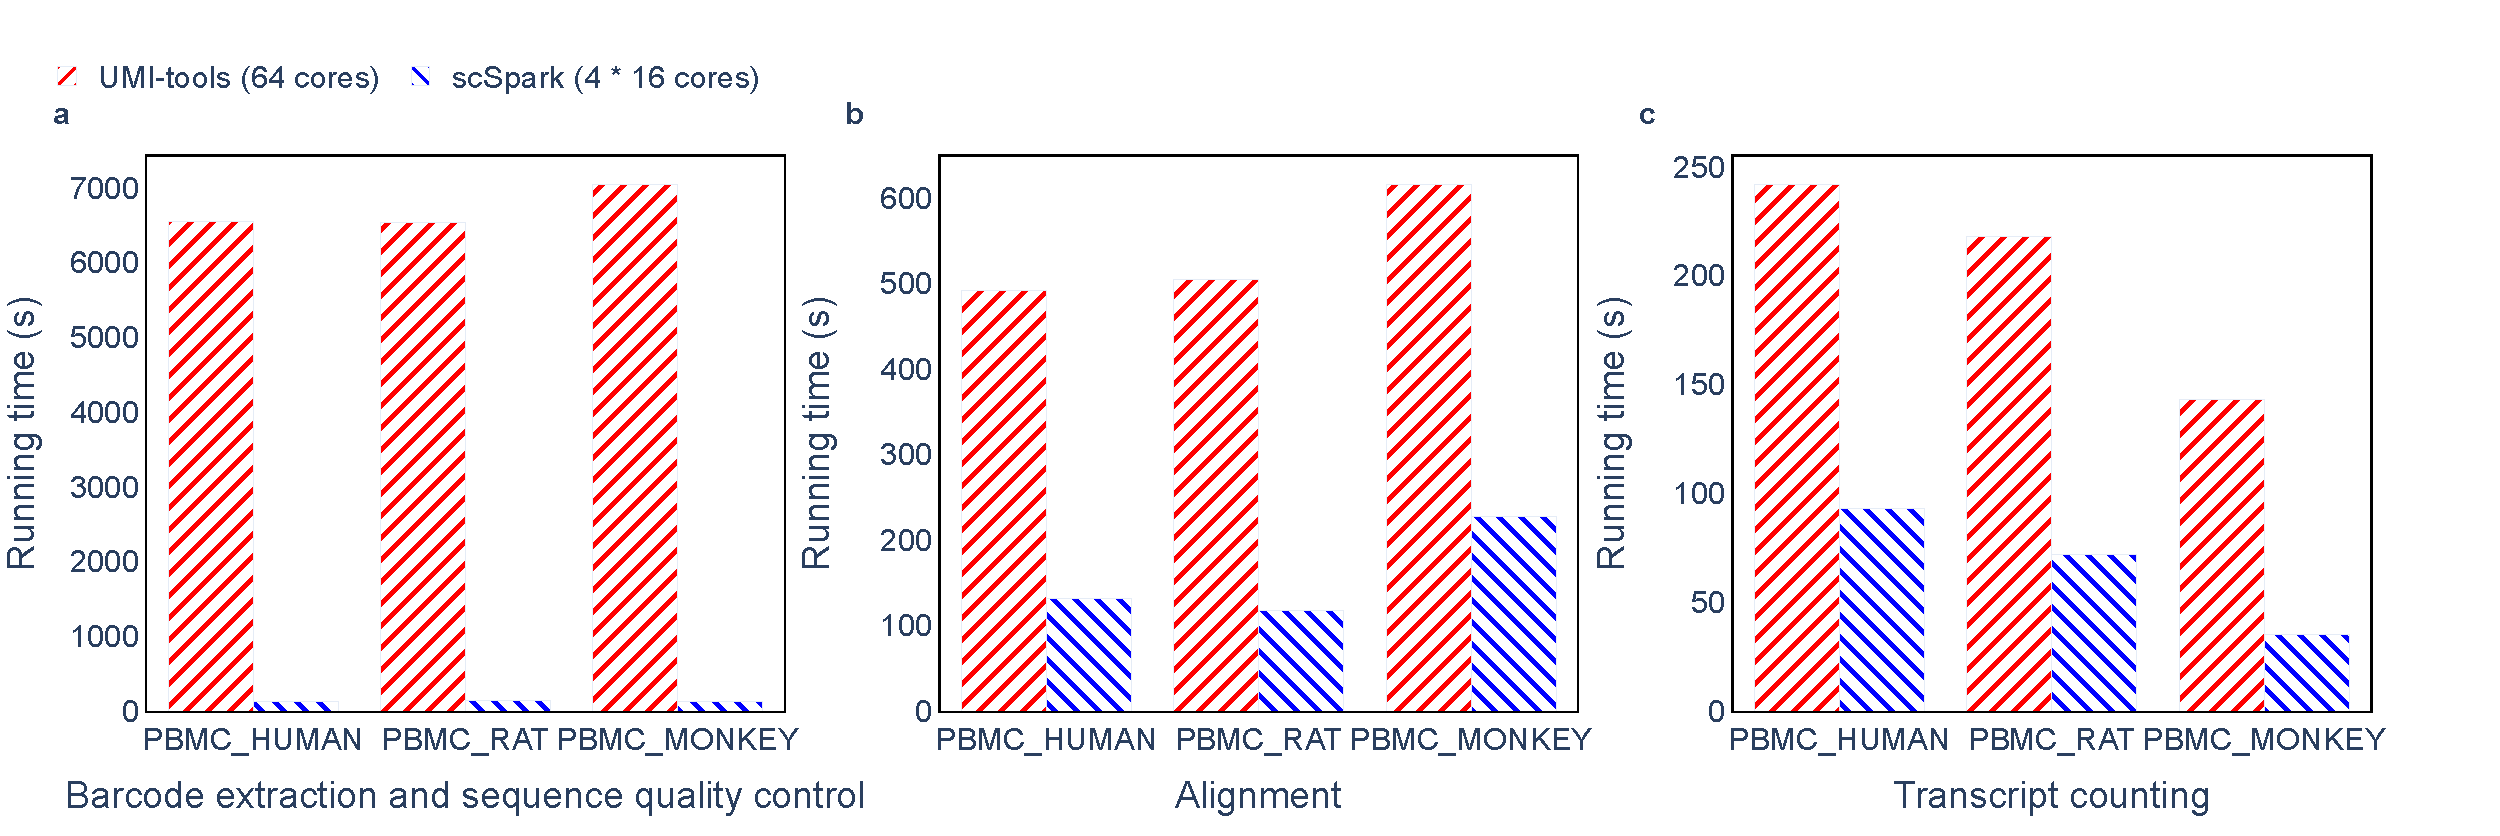
\includegraphics[width=0.5\textwidth]{fig2.pdf}
  \caption{New way to implement STAR's interface.} \label{fig2}
\end{figure}

Apart from Cellranger we can't know how it implements because it isn't an open source software. 
In previous pipeline, STAR needs to load extracted FASTQ R2 file or FASTQ R1 file. FASTQ R2 file and whitelist file will generate unneccessary disk access. 
We choose STAR as our aligner but avoid loading extracted FASTQ R2 and FASTQ R1 twice. 
As shown in Fig~\ref{fig2}, we utilized Java Native Interface to transfer extracted FASTQ R2 RDD's data to STAR program, and then run the STAR process.
The STAR aligner was encapsulated as a shared object and invoked the shared object as our aligner. 
To overcome imbalance problem of node's data volume, we repartitioned the extracted FASTQ R2 RDD, and then each node could run STAR parallelly with counterpoise data volume. 
We also found if node's in memory was enough, we could start up more than one STAR's in one node to achieve better parallel computing. 
The SAM or BAM file as STAR's output could generate more disk access waste than STAR's input. Here, we refered STAR-solo's solution to solve the problem by combining aligner and count. 
We used Java Native Interface again to transfer STAR results and directly abstract them to SAM RDD. 
This operation is parallel and totally in memory. 

\subsection{Count with multi-node}

\begin{figure}
  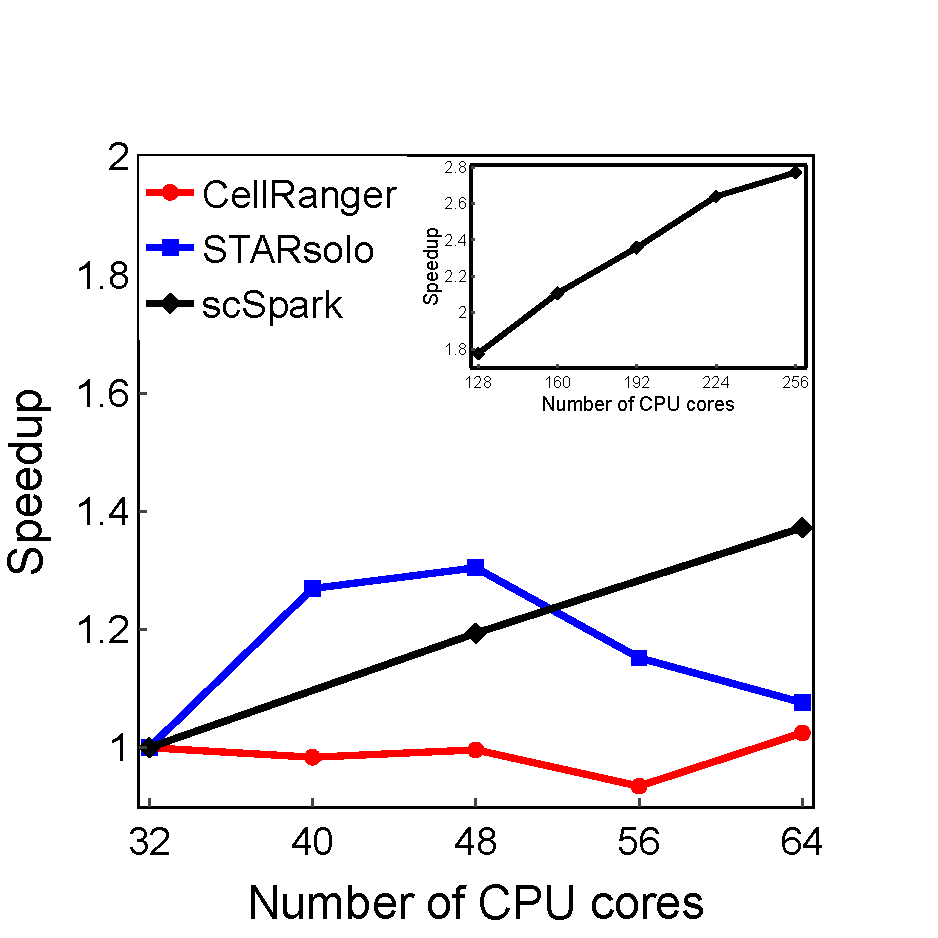
\includegraphics[width=0.5\textwidth]{fig3.pdf}
  \caption{An overview of Spark version count.} \label{fig3}
\end{figure}

As shown in Fig~\ref{fig3}, to take advantage of multi-node's compute capability, we used a new way to implement the count step. 
Except for SAM RDD that were generated in the previous step, we loaded GTF file to memory and abstract them as GTF RDD. 
Then we grouped SAM RDD and GTF RDD according to their cell name. 
Then we used flatMap function to parallelly compute each cell's read count. 
In the end, we collected results in all nodes, and the result files would produce the only output disk access in the whole program. 
ScSpark breaks the limitation of one node's computing and achieved large scalability. 

\section{Results}
We evaluated the speed and scalabilty for each step of scSpark to show the advantage of scSpark compared with the available pipelines. 

\subsection{Experimental environment and datasets}
We used Apache Spark version 2.1.0 as our in-memory computing environment.
The Spark cluster consists of Aliyun's ECS, and each node consists of 16 vCPU.
(Intel Xeon(Cascade Lake) Platinum 8269CY at 2.5GHz), 128 GBytes of DRAM and 400 GBits ESSD.

An example scRNA-seq dataset generated by 10X Genomics on their platform was used in our experiments.
10X-PBMC-10k dataset: 10X Genomics v3 10k peripheral blood mononuclear cell (PBMC) from a healthy donor~(\url{https://support.10xgenomics.com}).
It contains two gzipped FASTQ files. After unzipping, FASTQ R1's size is 69 Gbytes and FASTQ R2's size is 144 Gbytes. Each of the file contain 640 millions records.
We used STAR as our aligner, mapping to an index built on the human NCBI38 reference which called GRCh38.p12.genome.fa and use genome.gtf to filter the SAM~(\url{https://www.gencodegenes.org/human/releases.html}).
To evaluate the reason of why scSpark have a scalability ceiling and to experiment more convenient, we splitted FASTQ file to 100 millions, 160 millions and 320 millions records. 

\subsection{Efficiency evaluation}
\begin{table}
  \centering
  \caption{previous pipeline and scSpark's performance comparision}\label{tab1}
  \begin{tabular}{|l | l | l  l|}
  \hline
  System &  Cores & Spend time(s) \\
  \hline
   &  & 100M reads & 640M reads \\
  \hline
  UMI-tools & 64 cores & 7254 & 44160 \\
  \hline
  CellRanger & 64 cores & 6000 & 11700 \\
  \hline
  STAR-solo & 64 cores &  5820 & 8100 \\
  \hline
  scSpark & 4*16 cores & 354 & - \\
   & 8*16 cores & 210 & - \\
   & 16*16 cores & - & 841 \\
  \hline
  \end{tabular}
\end{table}
Limited by single machine's CPU cores, we only took 64 cores in preivous pipeline test.
Table~\ref{tab1} shown a summary of all the pipelines's performance.
We could see scSpark's speed is much more quick than any available pipeline in the same CPU cores environment.
And scSpark could get improvement when the cluster's CPU cores number increased.
\begin{table}
  \centering
  \caption{Performance comparision for each step}\label{tab2}
  \begin{tabular}{|l | l | l | l | l|}
  \hline
  System & Cores & filter & align & count \\
  \hline
  UMI-tools(100M reads) & 64 cores & 9720 & 600 & 1740 \\
  \hline
  UMI-tools (640M reads) & 64 cores & 33600 & 2160 & 8400 \\
  \hline
  scSpark (100M reads) & 4*16 cores & 31 & 270 & 53 \\
  \hline
  scSpark (640M reads) & 16*16 cores & 81 & 447 & 313 \\
  \hline
  \end{tabular}
\end{table}
Due to CellRanger isn't an open source software and STARsolo implements pipeline in a different way, we choose UMI-tools as scSpark each step's baseline.
As table~\ref{tab2} shown, scSpark is much faster than the previous pipeline in any single step.
We could see the most significant improvement came from the filtering step because we made a traditional single thread operation to parallelly computing in multi-machines and eliminates redundancy disk access.
For the same reason, scSpark's countting step also got considerable improvement.

\subsection{Scalability Evalution}
\begin{figure}
  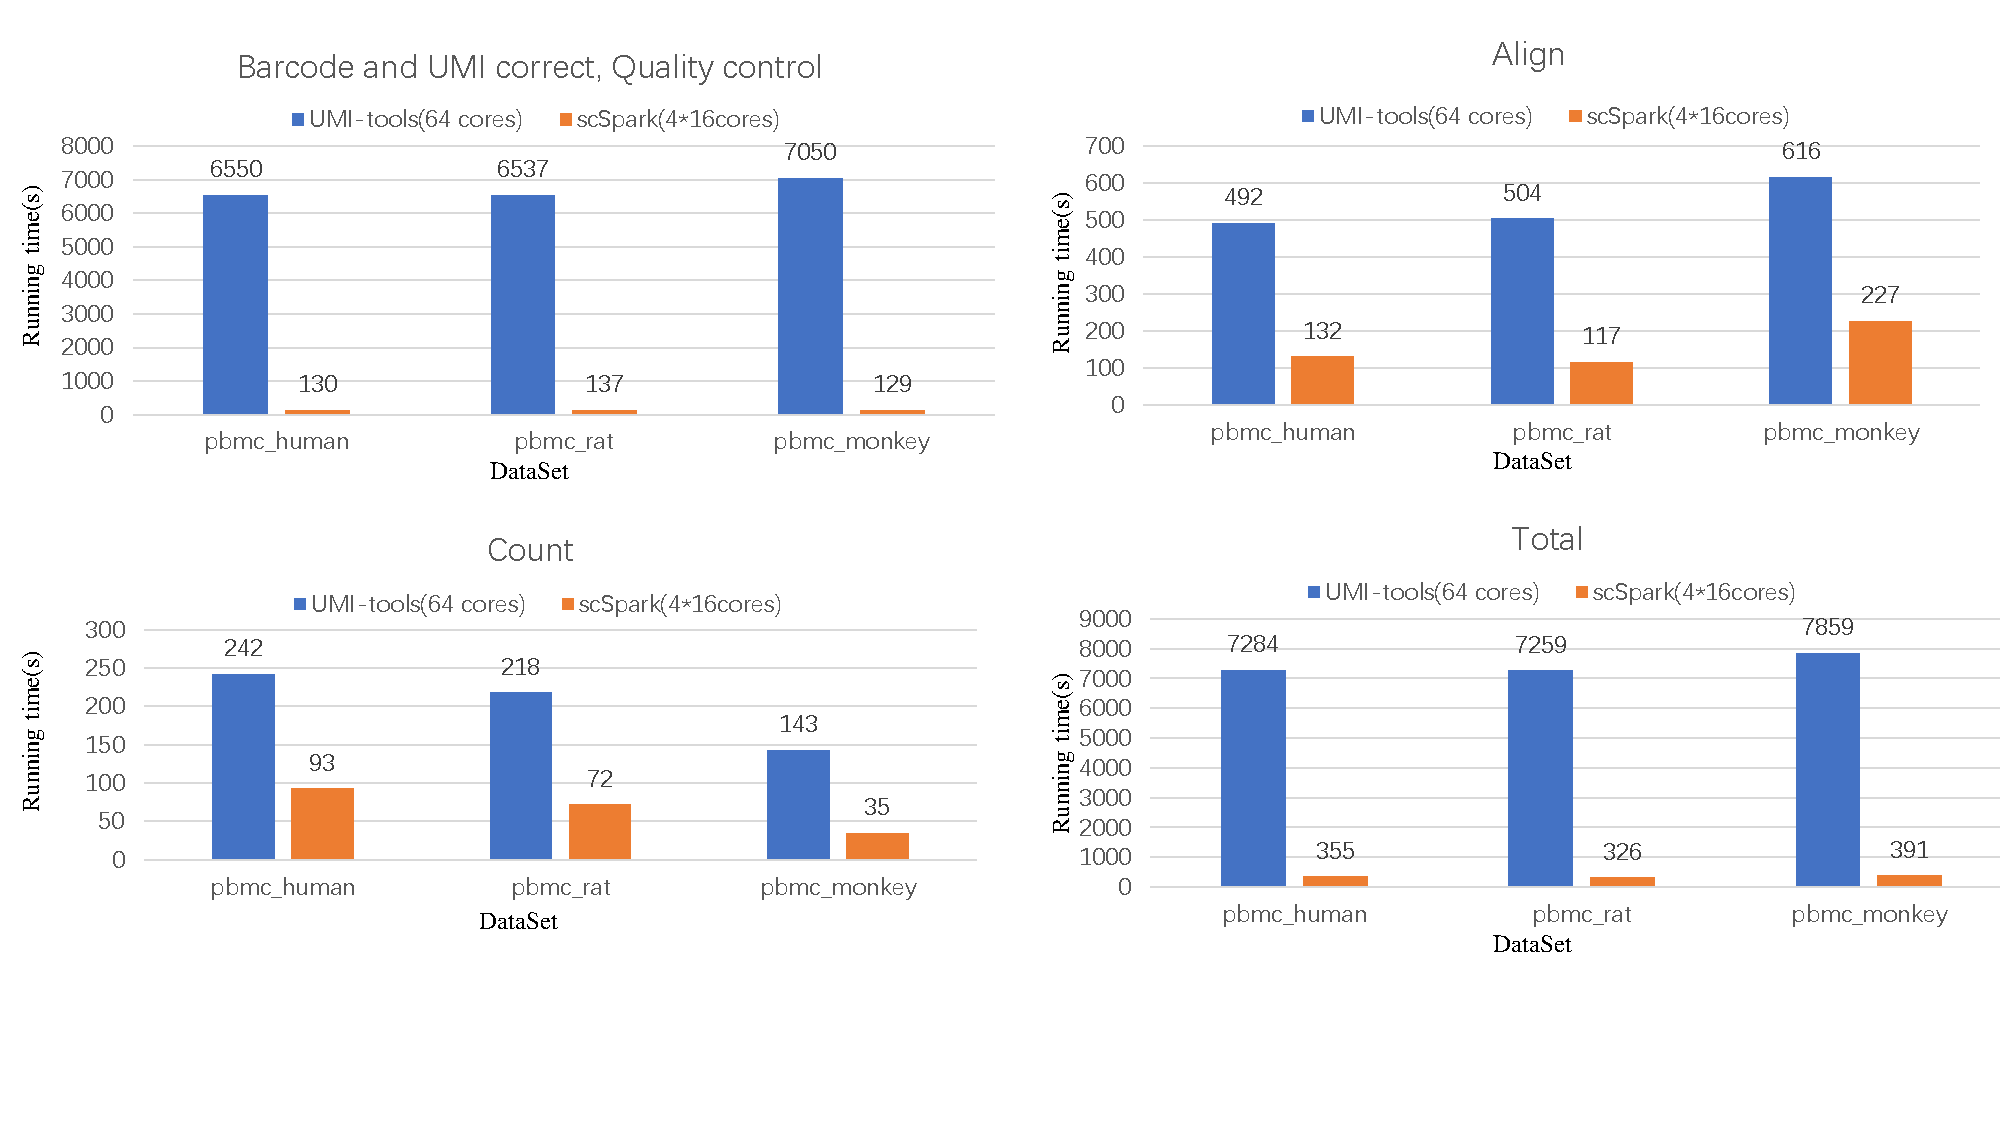
\includegraphics[width=0.5\textwidth]{fig4.pdf}
  \caption{Pipeline Scalability.} \label{fig4}
\end{figure}
ScSpark's second advantage is that it could get near linear improvement when the cluster's CPU core number increased. 
To test the scalability, we used 16 CPU cores performance as previous pipeline's baseline and 64 CPU cores performance as scSpark's baseline. 
We used a small sample which had 100 millions records to compare speedup. 
As shown in Fig~\ref{fig5}, we found that when CPU cores number increased, our program could get near linear speedup. 
In addition, we found if the CPU cores number exceeds a ceiling, both previous pipeline and scSpark will speedup nearly stop. 
Umi-tools did not show any scalabiliy and even a little slow down when the CPU cores number increased. 
STARsolo and CellRanger shown a little improve when the CPU cores increased to 32 from 16, but quickly stopped speedup. 
These results show that scSpark's scalability has great improvement. 

\subsection{Comparsion each step performance's increase}
\begin{figure}
  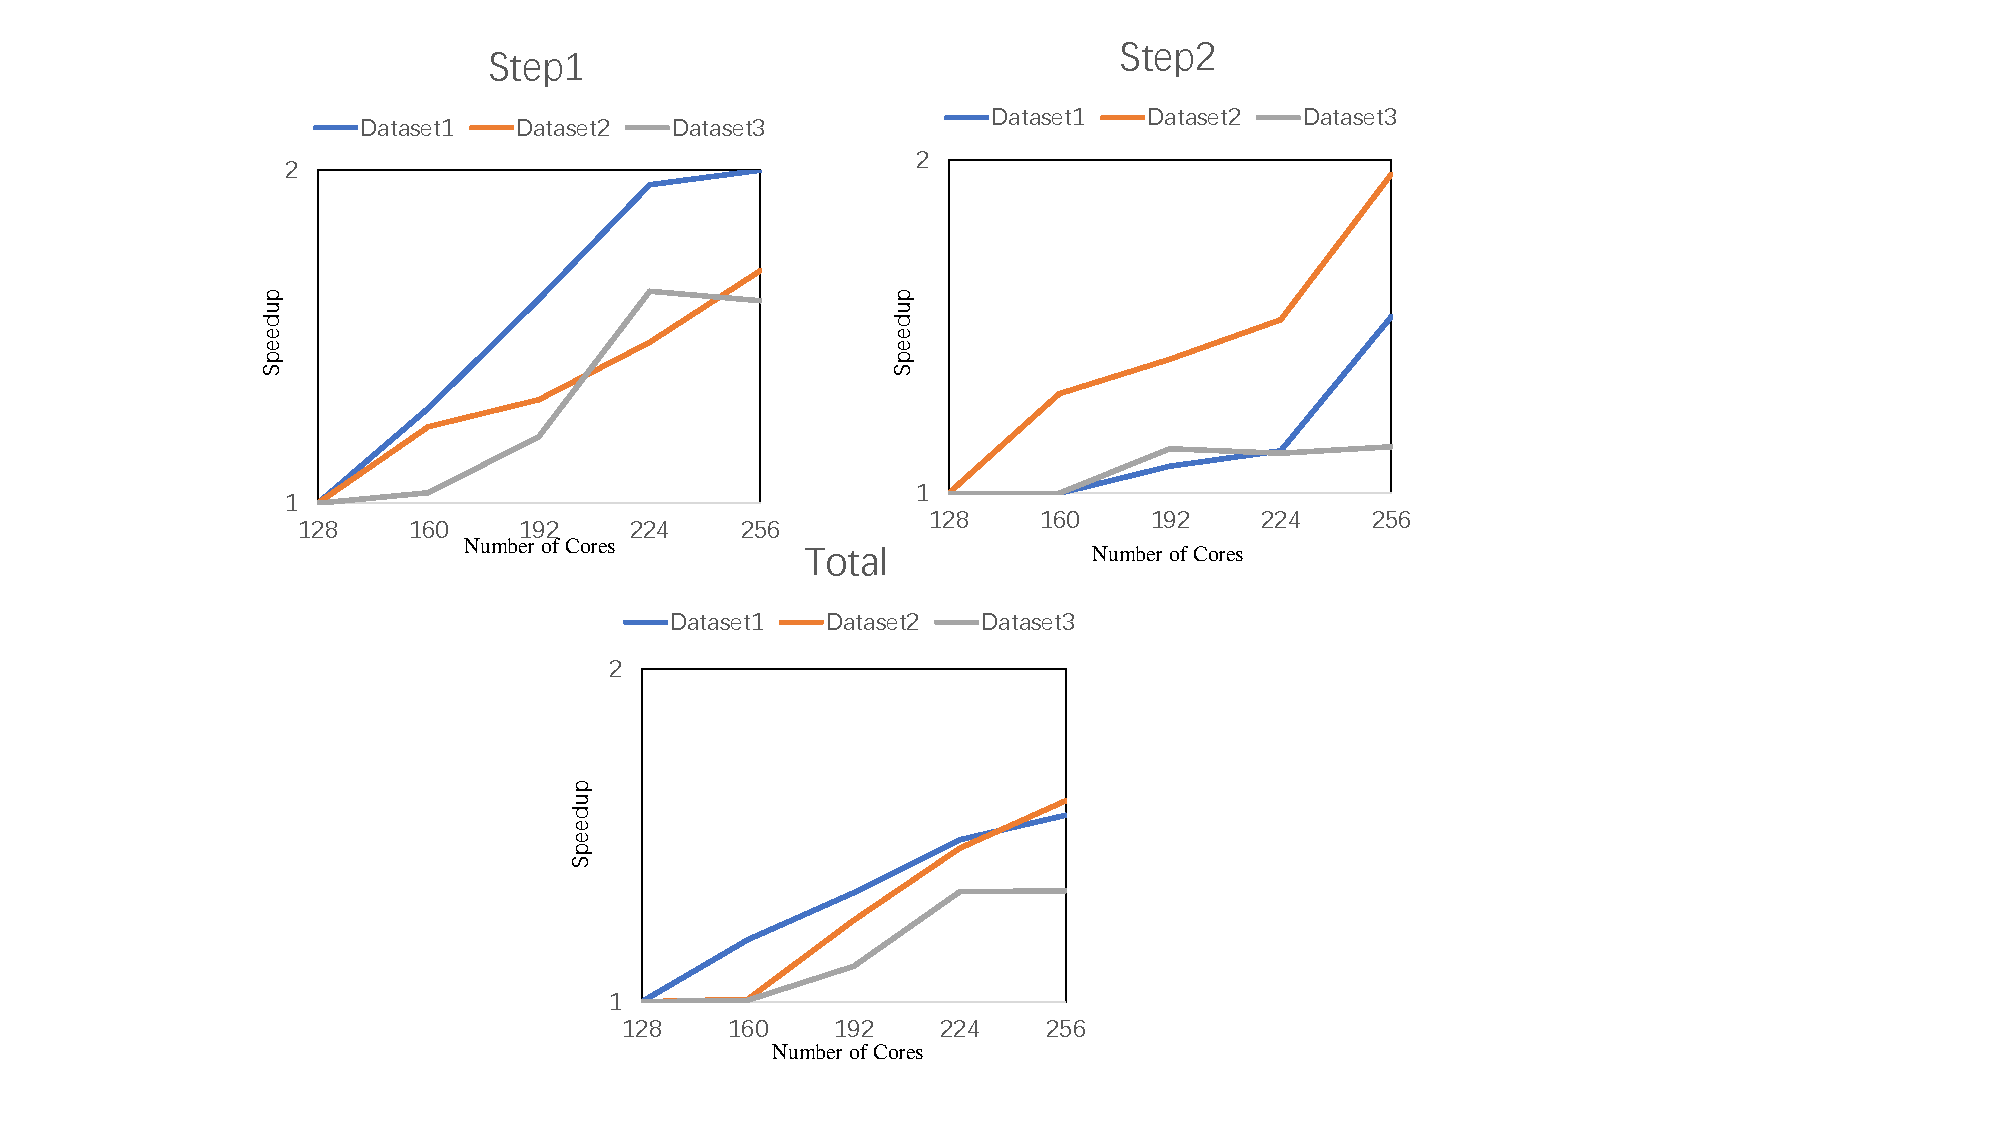
\includegraphics[width=0.5\textwidth]{fig5.pdf}
  \caption{Each step consumes time.} \label{fig5}
\end{figure}
We also recorded each step's process time to know the reason of the improvement.
As shown in Fig~\ref{fig5}, we found our program's scalability mainly came from the alignment step, which consumed most time in the whole program.
Next, we counted how much records scSpark's STAR program can process.
We found that, as shown in Fig~\ref{fig6}, STAR's mapping speed was influenced by the data size and dataset with small size will lost its scalability earier than those with large size.
\begin{figure}
  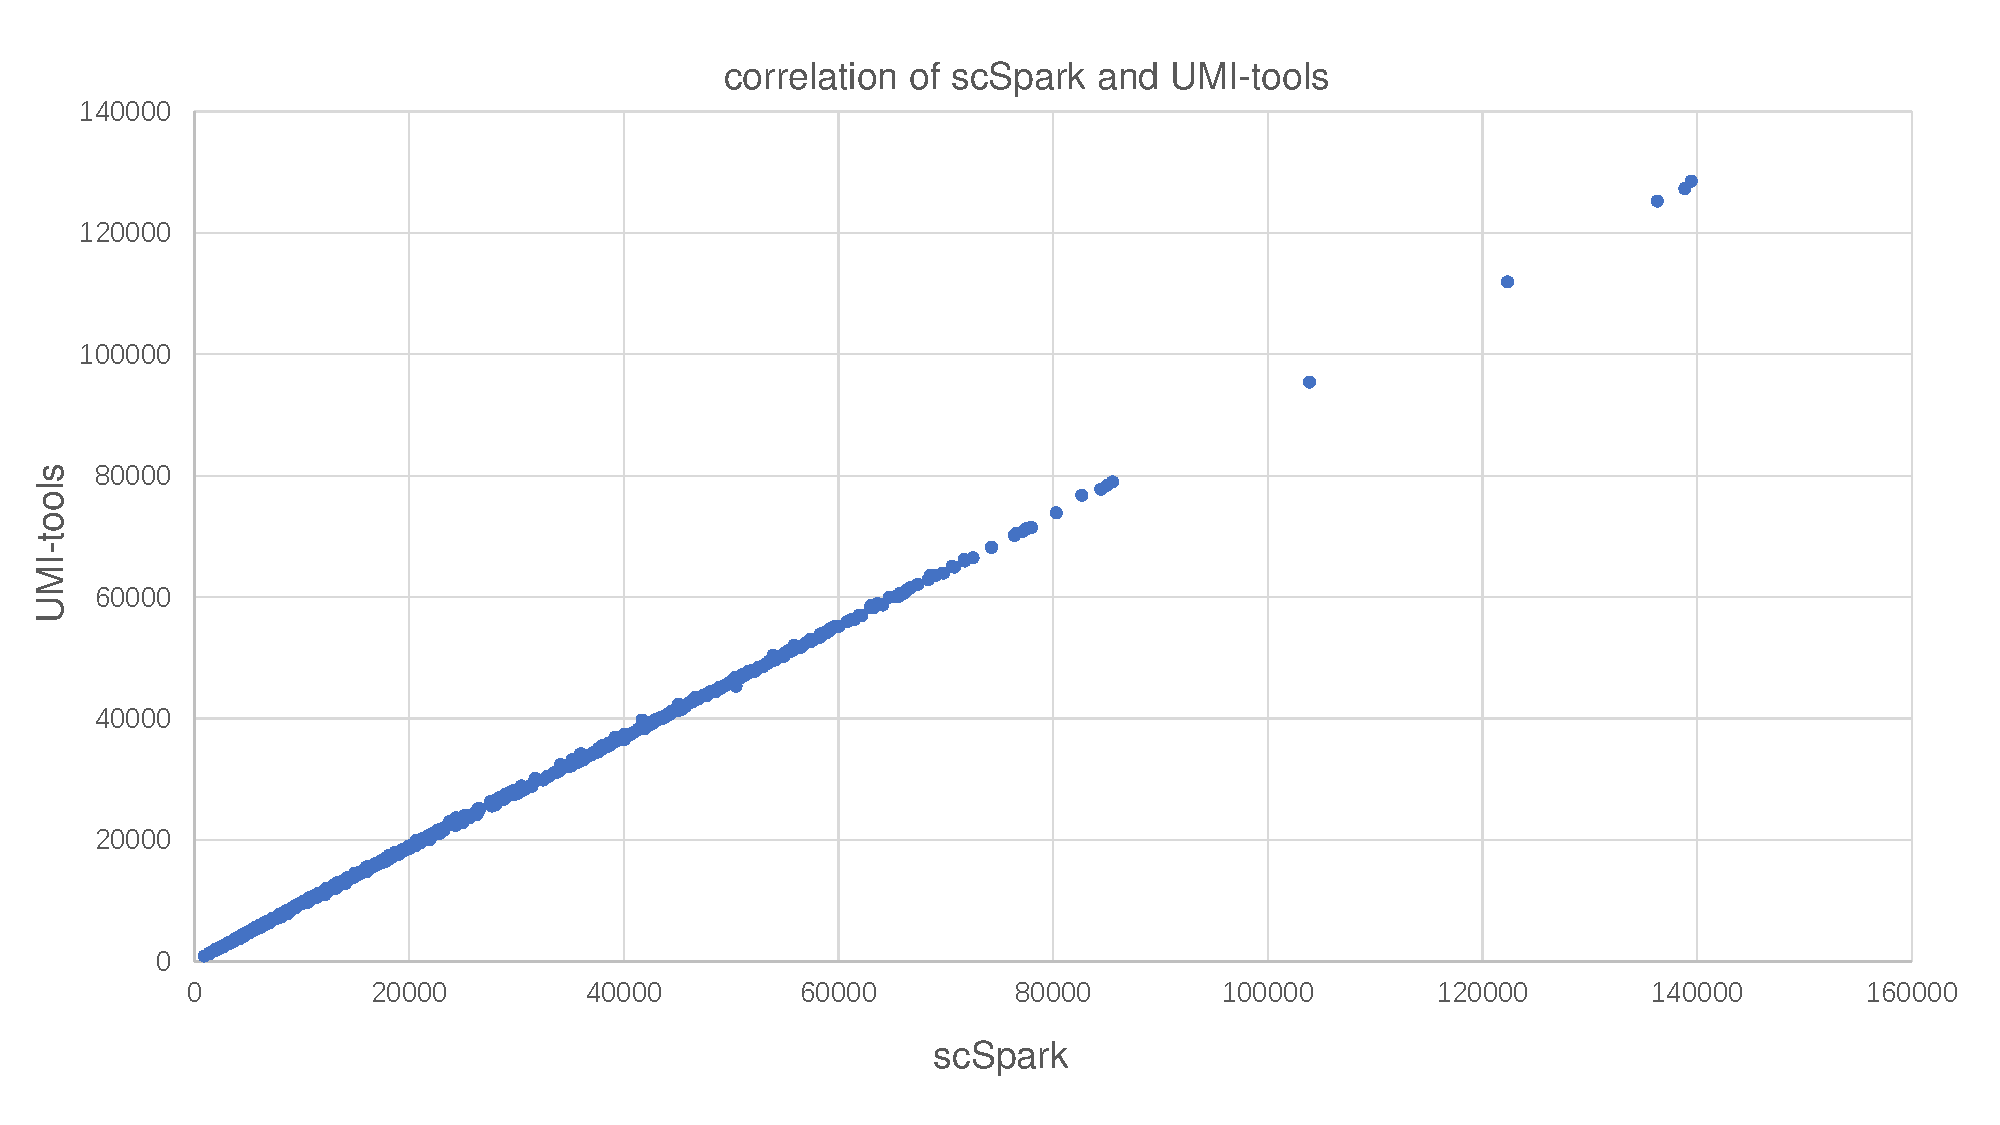
\includegraphics[width=0.5\textwidth]{fig6.pdf}
  \caption{Invoked STAR's mapping step.} \label{fig6}
\end{figure}

\begin{table}
    \centering
    \caption{Processing speed w.r.t. data size}\label{tab3}
    \begin{tabular}{|l | l | l | l | l|}
    \hline
    Volume (million reads) & 10 & 50 & 100 & 640 \\
    \hline
    Speed (million reads per hour) & 250.28 & 503.83 & 503.02 & 950 \\
    \hline
    \end{tabular}
  \end{table}
  
  Then we tested STAR program, and found the mapping speed was also influenced by data size. 
  As Table~\ref{tab3} shown, the speed of STAR mapping increased when the size of data increase. 
  So when we got scalability by increasing partition, each partition's read number decreased and it would limit the scalability improvement. 
  
  \subsection{Performance Analysis}
  We tested performance to find the bottleneck of scSpark.
  We used 640 millions records of FASTQ data to evaluate two aspects of scSpark.
  First we compared network shuffle and disk access spend by scSpark and compute proportions of time, which helped to find whether network shuffle or disk access occupies too much time.
  Secondy, we tested CPU and memory usage, to ensure which resources would cause scSpark's bottleneck.
  
  \subsubsection{Network and disk behavior}
  \begin{figure}
    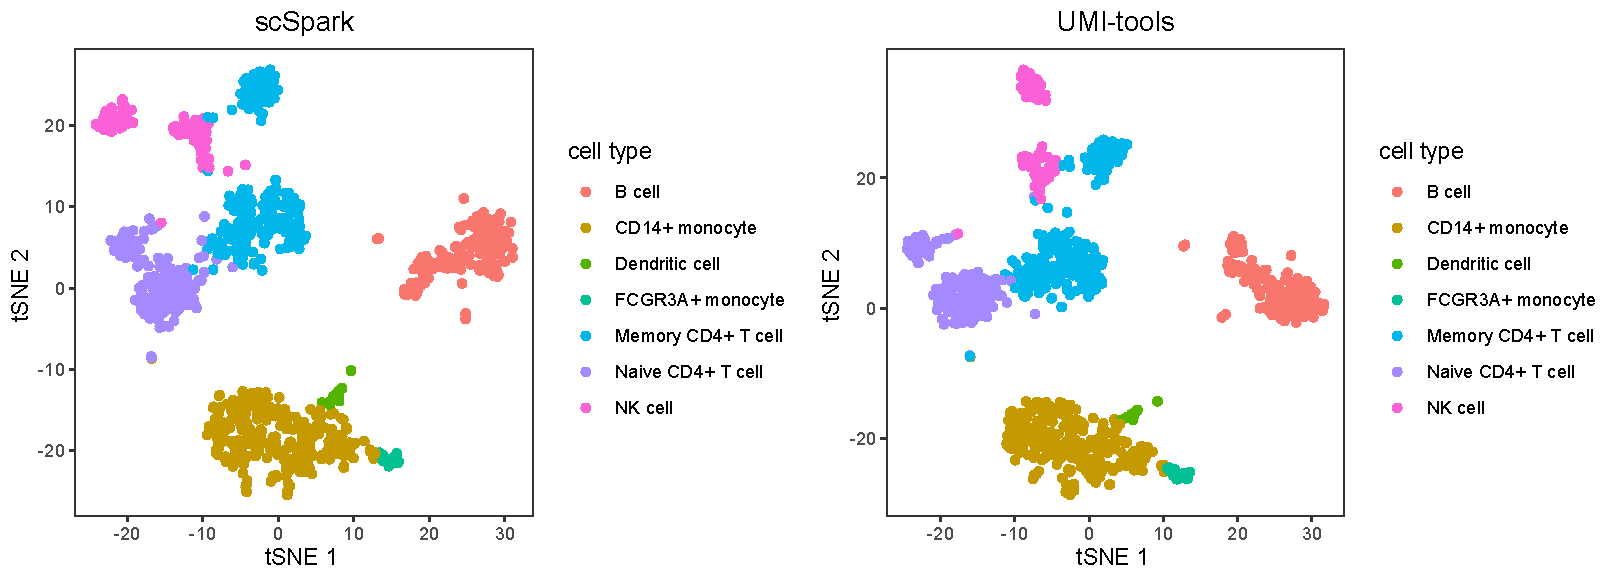
\includegraphics[width=0.5\textwidth]{fig7.pdf}
    \caption{Each step consumes time.} \label{fig7}
  \end{figure}
  We computed network time by summing up the time that our scSpark shuffle data in multi machine. 
  Disk access comes from loading FASTQ, STAR's index and GTF files. 
  The ideal situation is tasks did not waste any time in disk access and network shuffle. 
  We found that scSpark's computing time occupied most execute time. 
  Except STAR's index file, all files' disk access distributed to each node would improve whole system's loading speed. 
  And we found the time that waste in shuffling doesn't occupy too much time. 
  
  \subsubsection{CPU and memory usage}
  \begin{figure}
    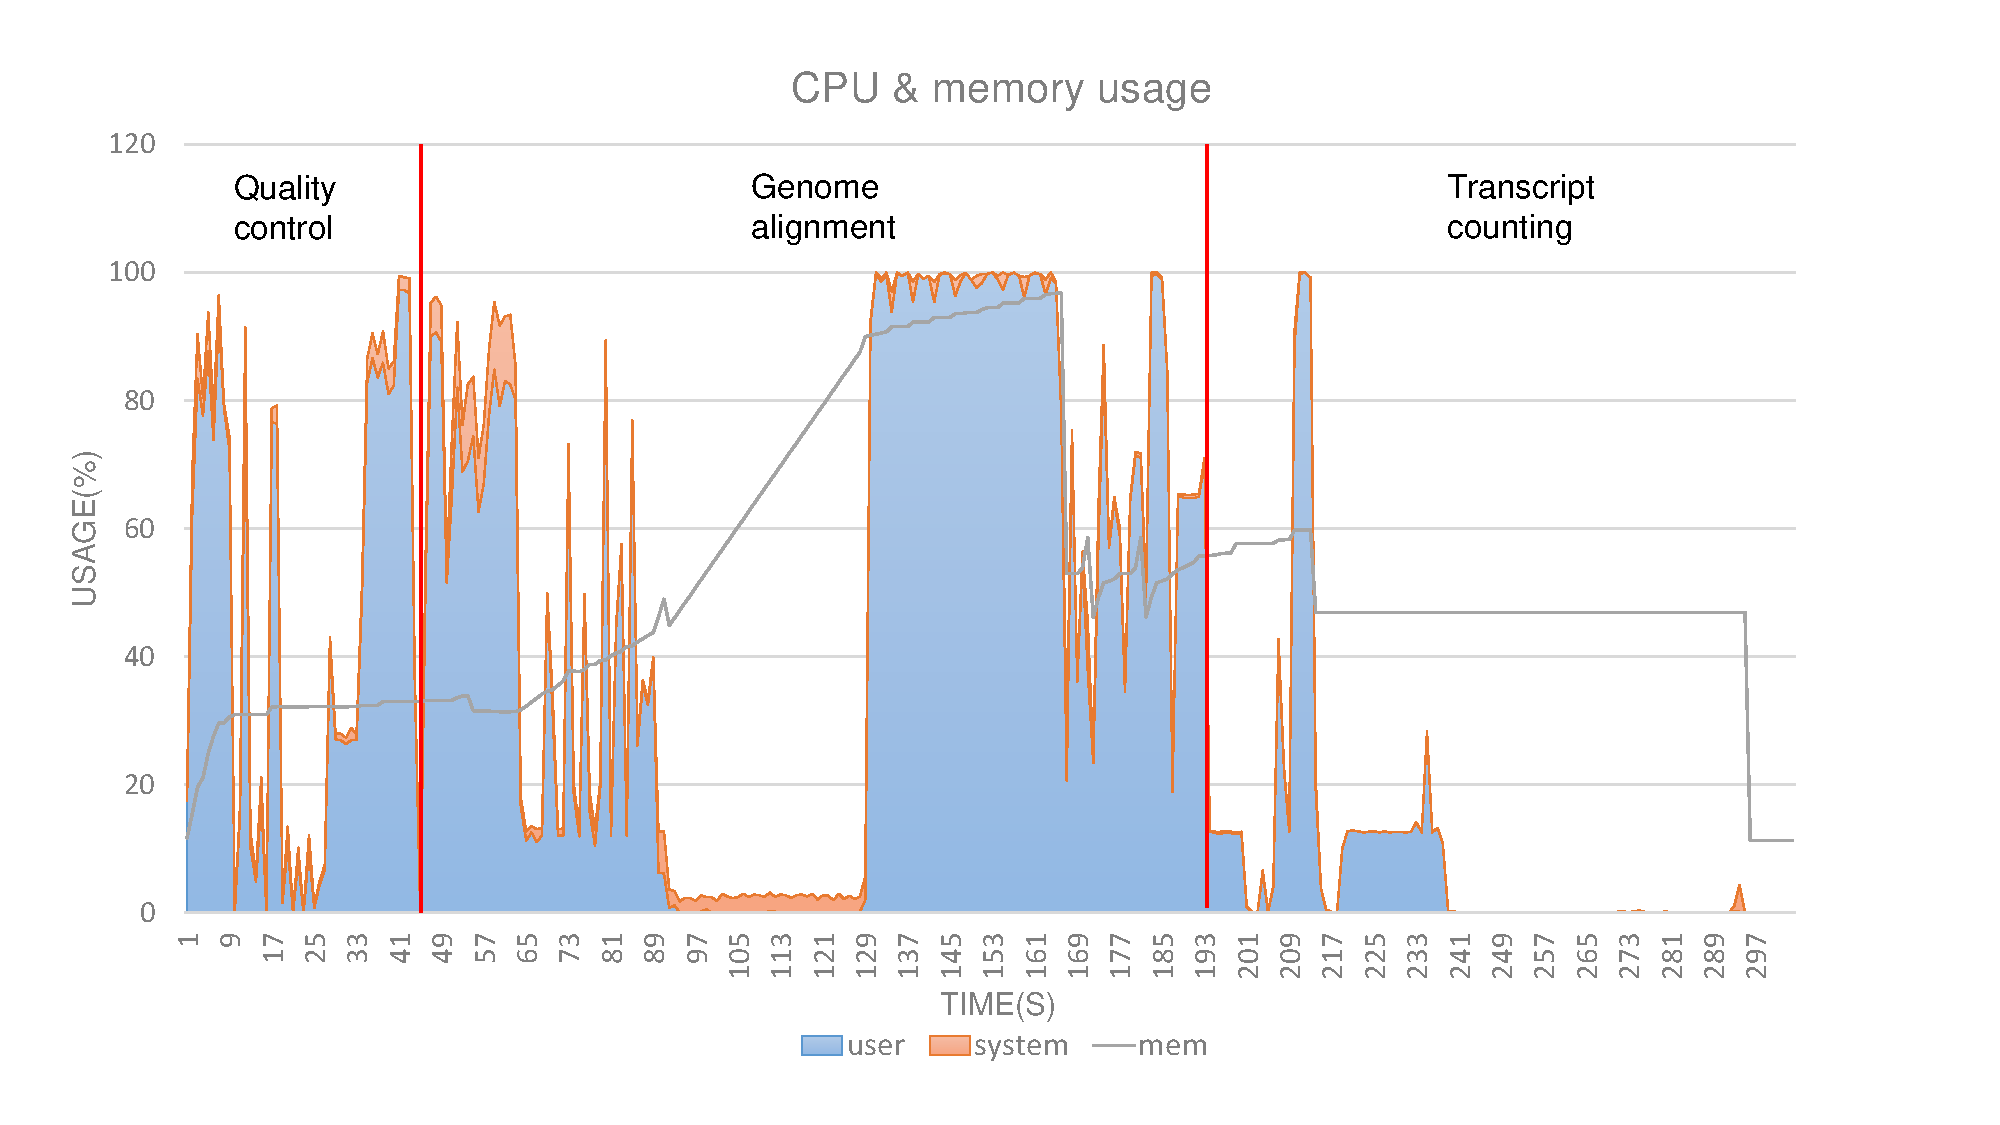
\includegraphics[width=0.5\textwidth]{fig8.pdf}
    \caption{CPU and Memory usage of scSpark.} \label{fig8}
  \end{figure}
  We monitored scSpark's CPU and memory usage during processing. 
  As Fig~\ref{fig8} shown, in sequence quality control step, scSpark highly exploited each node's multi cores CPU to achieve speedup. 
  Other pipelines' single thread solution's CPU usage is much lower than scSpark. 
  We found that scSpark's boundary mainly came from genome alignment.
  Because we invoked STAR as our alignment tool, and STAR's program naturally occupy most proportion of memory in this step.
  
  \subsubsection{Biological verification}
  ScSpark is developed based on UMI-tools, which has been fully verified in terms of accuracy. 
  This section we used the gene expression matrix obtained by scSpark and UMI-tools to perform downstream analysis of scRNA-seq data. 
  We compared transcript counting results and clusters of cells in the hgmm-1k-v3 dataset to verify the correlation between scSpark and UMI-tools. 
  
  As Fig~\ref{fig9} shown, for each after processing cell barcode, we compared our scSpark's result with UMI-tools' result, their gene expression matrix approximate fit $y=x$, $R^{2}$ closed to 0.9998. 
  \begin{figure}
    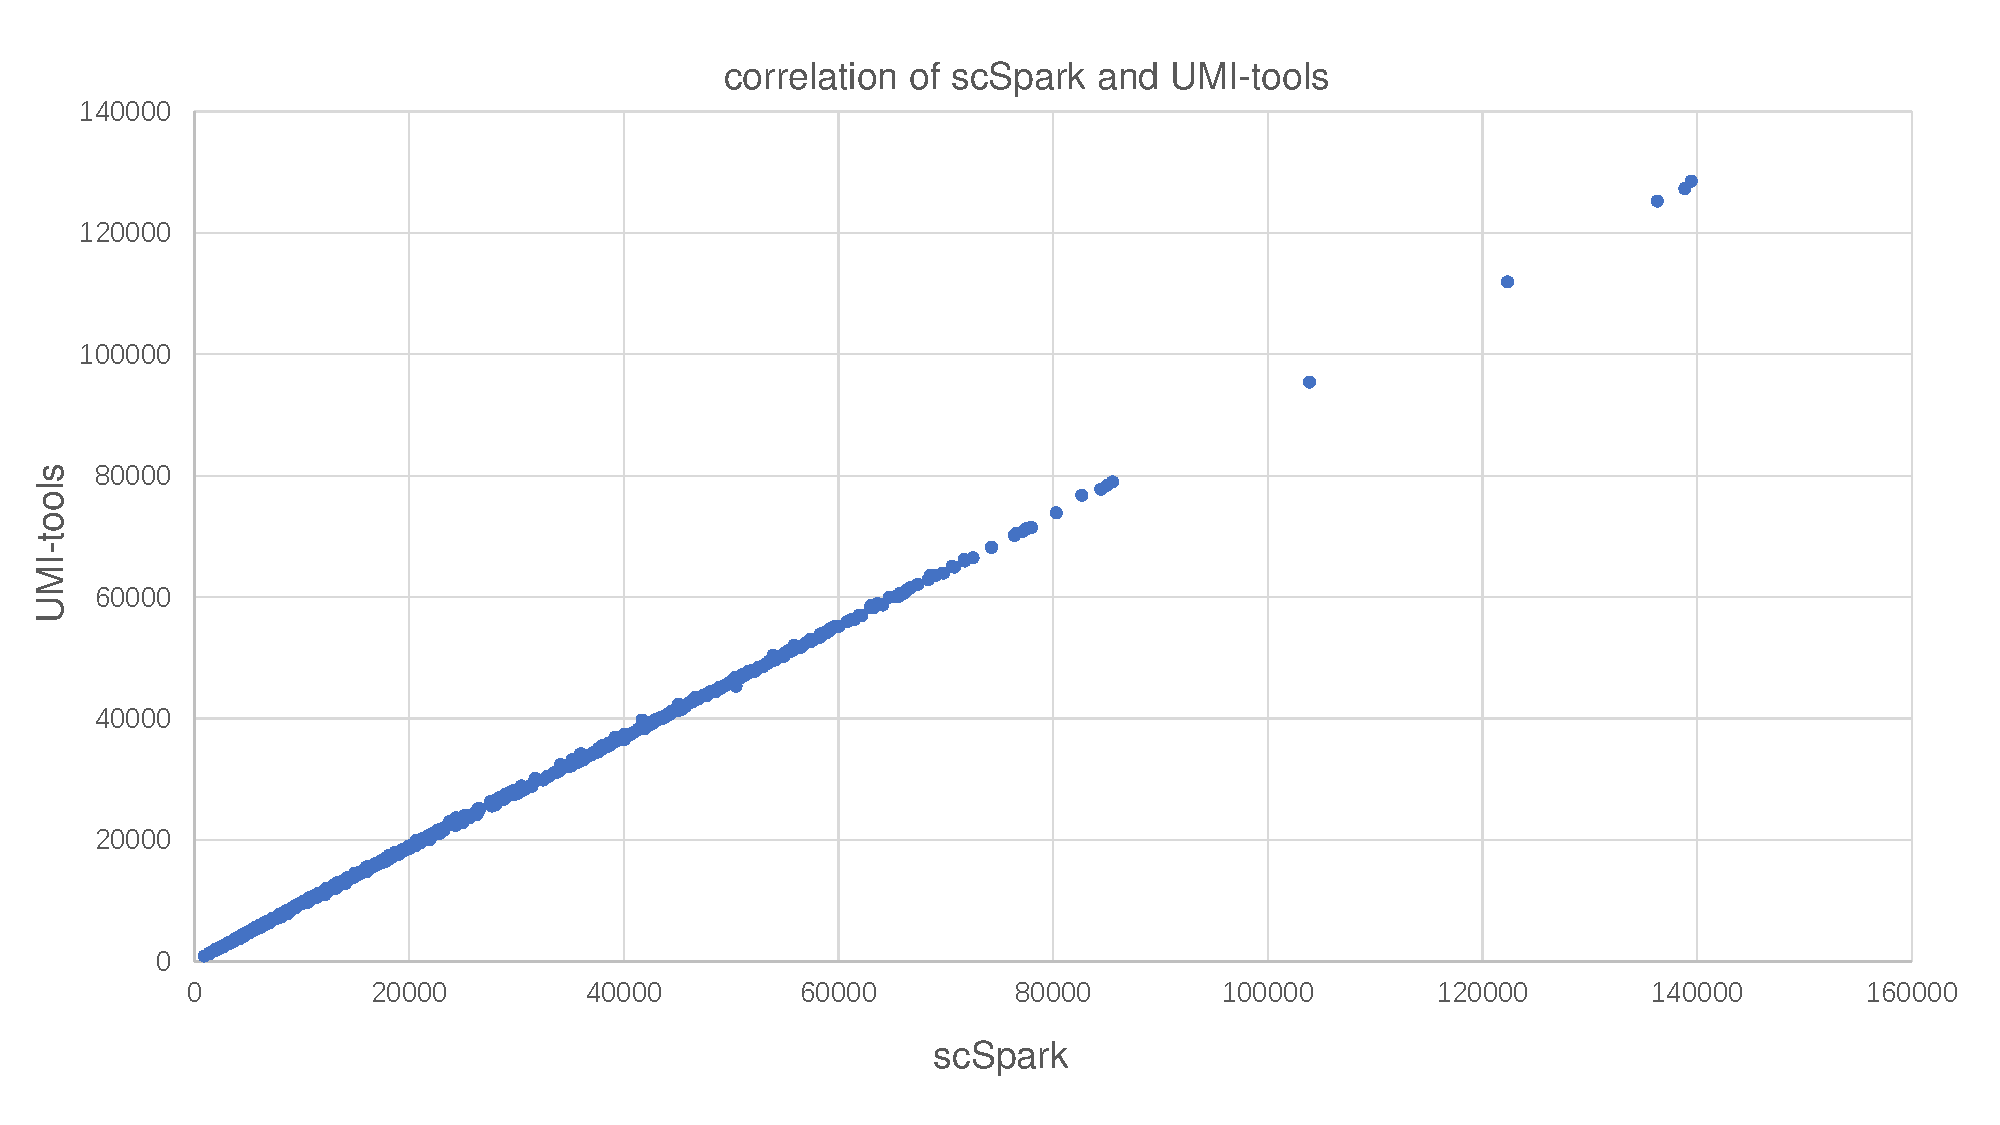
\includegraphics[width=0.5\textwidth]{fig9.pdf}
    \caption{The correlation of transcript counting results for scSpark and UMI-tools.} \label{fig9}
  \end{figure}
  Furthermore, we used Seurat to obtain tSNE plots for the visualization of cell clusters. 
  And as Fig~\ref{fig10} shown, the overlapping frequence of cell clustering results were 【?】.【这里没有用相关性计算,可以计算每个细胞亚群的
  \begin{figure*}
    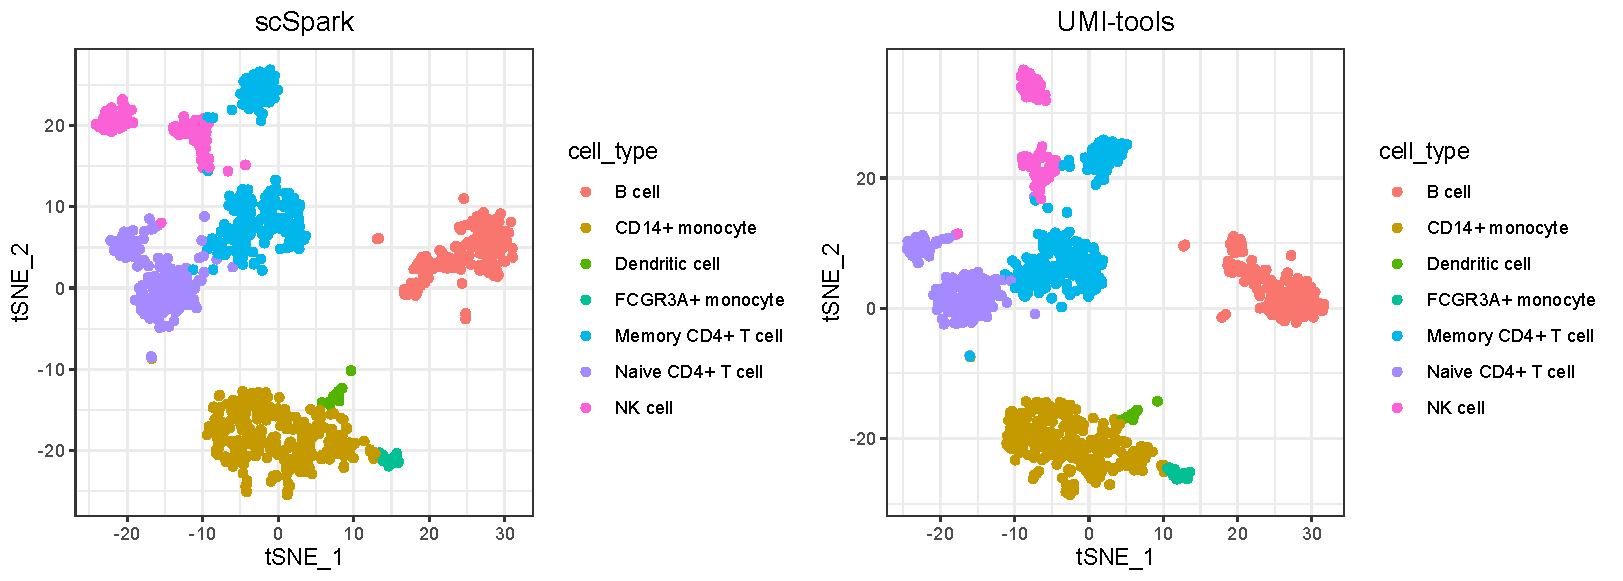
\includegraphics[width=\textwidth]{fig10.pdf}
    \caption{tSNE plots based on scSpark and UMI-tools' gene expression matrices.} \label{fig10}
  \end{figure*}
  \section{Conclusion}
  In this paper, we proposed a way to utilize Apache Spark's in memory compute trait and achieved considerable speedup and scalability. 
  Our scSpark can take advantages of multi-machine compute capacity to speedup key steps of scRNA-seq preprocessing and eliminate redundant disk access. 
  
  In addition to performance improvement, scSpark also show much more scalable than any previous pipeline and its speed closes to linear improvement.
  Moreover,scSpark can improve scalability by increasing partition number if the resource is sufficient.
  
  And we also found our scSpark's scalability improvement has a ceiling. 
  The reason is that our scSpark invokes STAR's mapping speed, which is influenced by loading index time. 
  And if data size is tiny, the influence occupies a large proportion of whole the STAR program process time. 

% \section*{Acknowledgment}

% The preferred spelling of the word ``acknowledgment'' in America is without 
% an ``e'' after the ``g''. Avoid the stilted expression ``one of us (R. B. 
% G.) thanks $\ldots$''. Instead, try ``R. B. G. thanks$\ldots$''. Put sponsor 
% acknowledgments in the unnumbered footnote on the first page.

% \section*{References}

% Please number citations consecutively within brackets \cite{b1}. The 
% sentence punctuation follows the bracket \cite{b2}. Refer simply to the reference 
% number, as in \cite{b3}---do not use ``Ref. \cite{b3}'' or ``reference \cite{b3}'' except at 
% the beginning of a sentence: ``Reference \cite{b3} was the first $\ldots$''

% Number footnotes separately in superscripts. Place the actual footnote at 
% the bottom of the column in which it was cited. Do not put footnotes in the 
% abstract or reference list. Use letters for table footnotes.

% Unless there are six authors or more give all authors' names; do not use 
% ``et al.''. Papers that have not been published, even if they have been 
% submitted for publication, should be cited as ``unpublished'' \cite{b4}. Papers 
% that have been accepted for publication should be cited as ``in press'' \cite{b5}. 
% Capitalize only the first word in a paper title, except for proper nouns and 
% element symbols.

% For papers published in translation journals, please give the English 
% citation first, followed by the original foreign-language citation \cite{b6}.

\bibliographystyle{IEEEtran}
\bibliography{reference}

% \begin{thebibliography}{00}
% \bibitem{b1} G. Eason, B. Noble, and I. N. Sneddon, ``On certain integrals of Lipschitz-Hankel type involving products of Bessel functions,'' Phil. Trans. Roy. Soc. London, vol. A247, pp. 529--551, April 1955.
% \bibitem{b2} J. Clerk Maxwell, A Treatise on Electricity and Magnetism, 3rd ed., vol. 2. Oxford: Clarendon, 1892, pp.68--73.
% \bibitem{b3} I. S. Jacobs and C. P. Bean, ``Fine particles, thin films and exchange anisotropy,'' in Magnetism, vol. III, G. T. Rado and H. Suhl, Eds. New York: Academic, 1963, pp. 271--350.
% \bibitem{b4} K. Elissa, ``Title of paper if known,'' unpublished.
% \bibitem{b5} R. Nicole, ``Title of paper with only first word capitalized,'' J. Name Stand. Abbrev., in press.
% \bibitem{b6} Y. Yorozu, M. Hirano, K. Oka, and Y. Tagawa, ``Electron spectroscopy studies on magneto-optical media and plastic substrate interface,'' IEEE Transl. J. Magn. Japan, vol. 2, pp. 740--741, August 1987 [Digests 9th Annual Conf. Magnetics Japan, p. 301, 1982].
% \bibitem{b7} M. Young, The Technical Writer's Handbook. Mill Valley, CA: University Science, 1989.
% \end{thebibliography}
% \vspace{12pt}
% \color{red}
% IEEE conference templates contain guidance text for composing and formatting conference papers. Please ensure that all template text is removed from your conference paper prior to submission to the conference. Failure to remove the template text from your paper may result in your paper not being published.

\end{document}
